%図や表現の確認
\chapter{音楽用語の定義}

本章では音楽用語の定義及びその説明を行う。

\section{音}

音とは、弾性体~(空気)~中を伝播する弾性波により起こされる音波が聴覚により感じられるもののことである。また、音波に周期性があり明確な音程を持つ音として聞こえる場合は楽音と呼ばれる。

\section{楽音の三要素}

楽音は高さ,大きさ,音色の三つの要素~(音の三要素)~から成り立ち、人間はこれらを知覚することができる。また、本論文では楽音のことを音と呼ぶ。

\subsection{音の高さ}

\begin{figure}[ht]
\begin{center}
\begin{minipage}{0.48\hsize}
\begin{center}
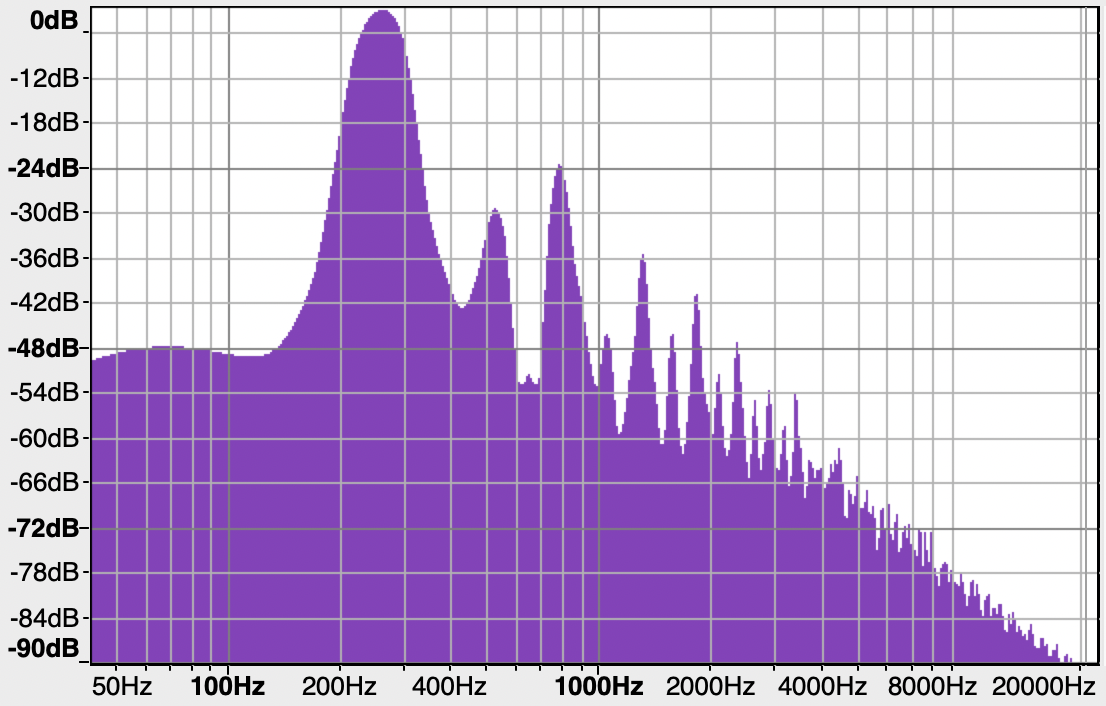
\includegraphics[width=0.95\hsize]{figure/c4_harp_spectrum.png}
\caption{音波の周波数スペクトル}
\label{fig:spectrum}
\end{center}
\end{minipage}
\begin{minipage}{0.48\hsize}
\begin{center}
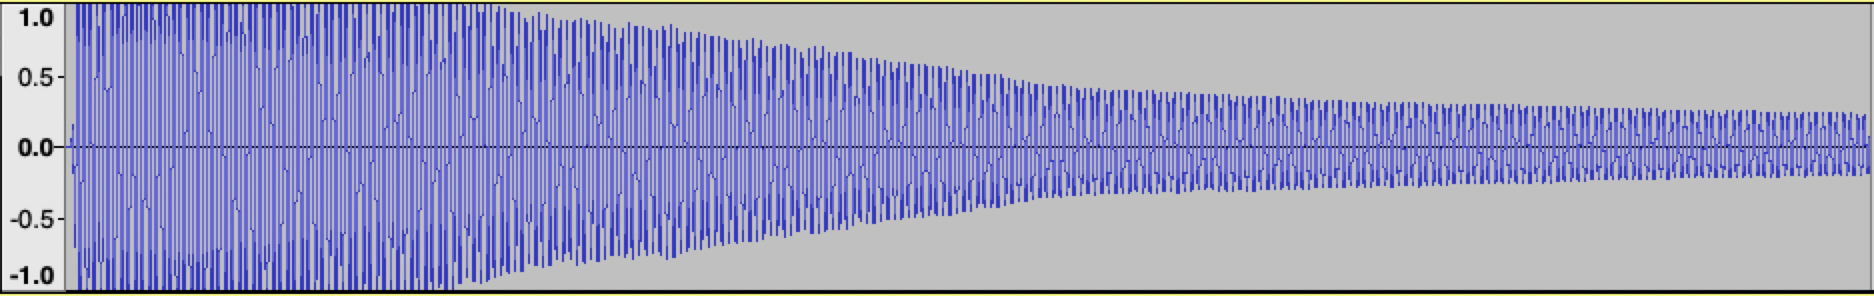
\includegraphics[width=0.95\hsize]{figure/c4_harp_wav.png}
\caption{音波の波形}
\label{fig:wav}
\end{center}
\end{minipage}
\end{center}
\end{figure}

音の高さは音波の周波数により決まる。人間には周波数が高い音は高く、周波数が低い音は低く知覚さる。また、複数の周波数の音波が音に含まれる場合は最も低い周波数成分の音波~(基音)~を音の高さとして知覚する。

図\ref{fig:spectrum}は図\ref{fig:wav}で示される音波にフーリエ変換を行うことで求められる周波数スペクトルである。周波数スペクトルはそれぞれの周波数成分がどれだけその音波に含まれているかを示すので、この音波の基音は264Hzであることがわかる。

\subsection{音の大きさ}

\begin{figure}[ht]
\begin{center}
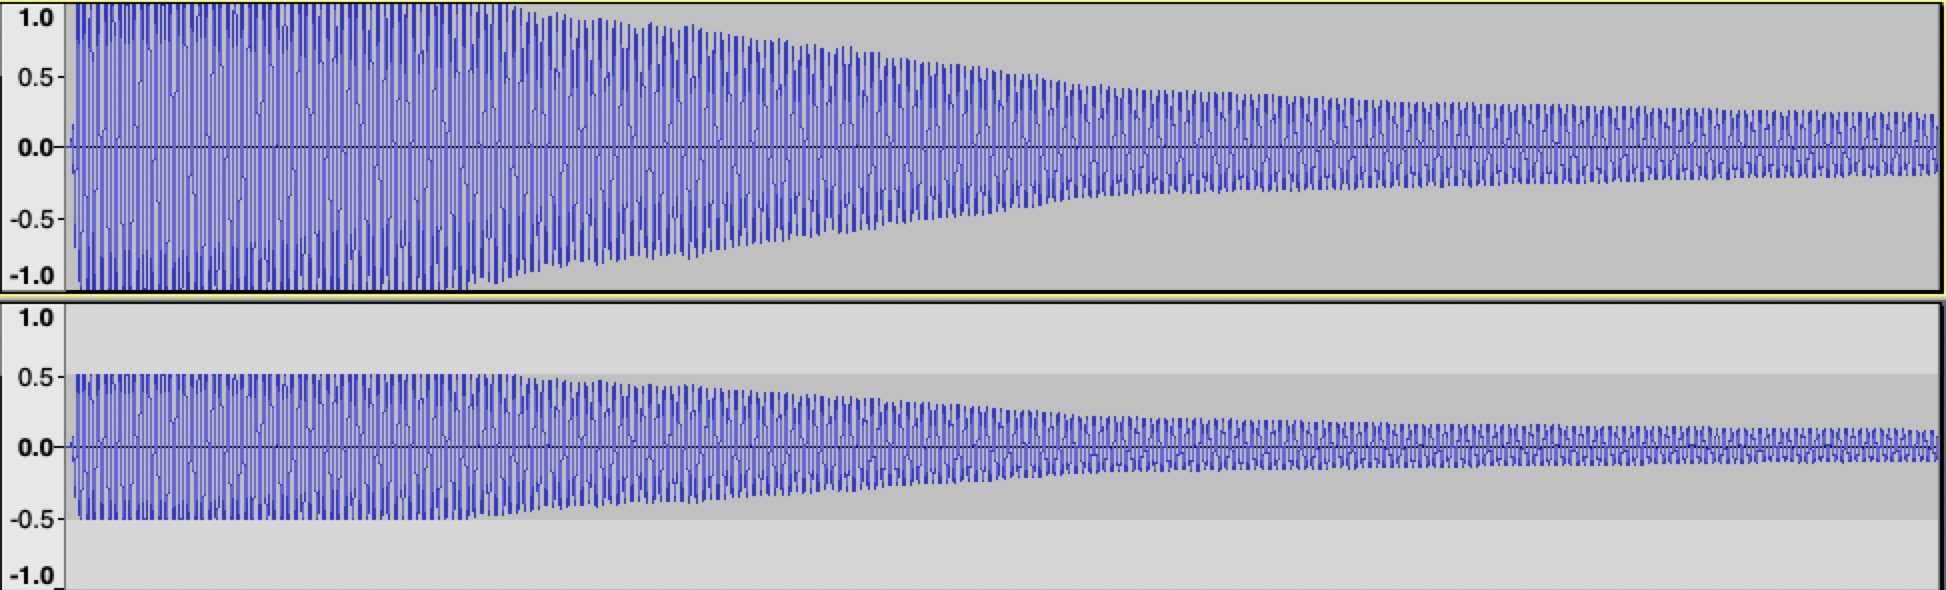
\includegraphics[width=0.7\hsize]{figure/c4_harp_loudness.png}
\caption{音の大きさの異なる音波}
\label{fig:loudness}
\end{center}
\end{figure}

音の大きさは音波の振幅により決まる。人間には振幅が大きい音は大きく、振幅が小さい音は小さく知覚さる。

図\ref{fig:loudness}では、同じ楽器から出る同じ高さの音の音波を示しており、振幅の大きい後者の方が大きい音として人間には知覚される。

\subsection{音の音色}

\begin{figure}[ht]
\begin{center}
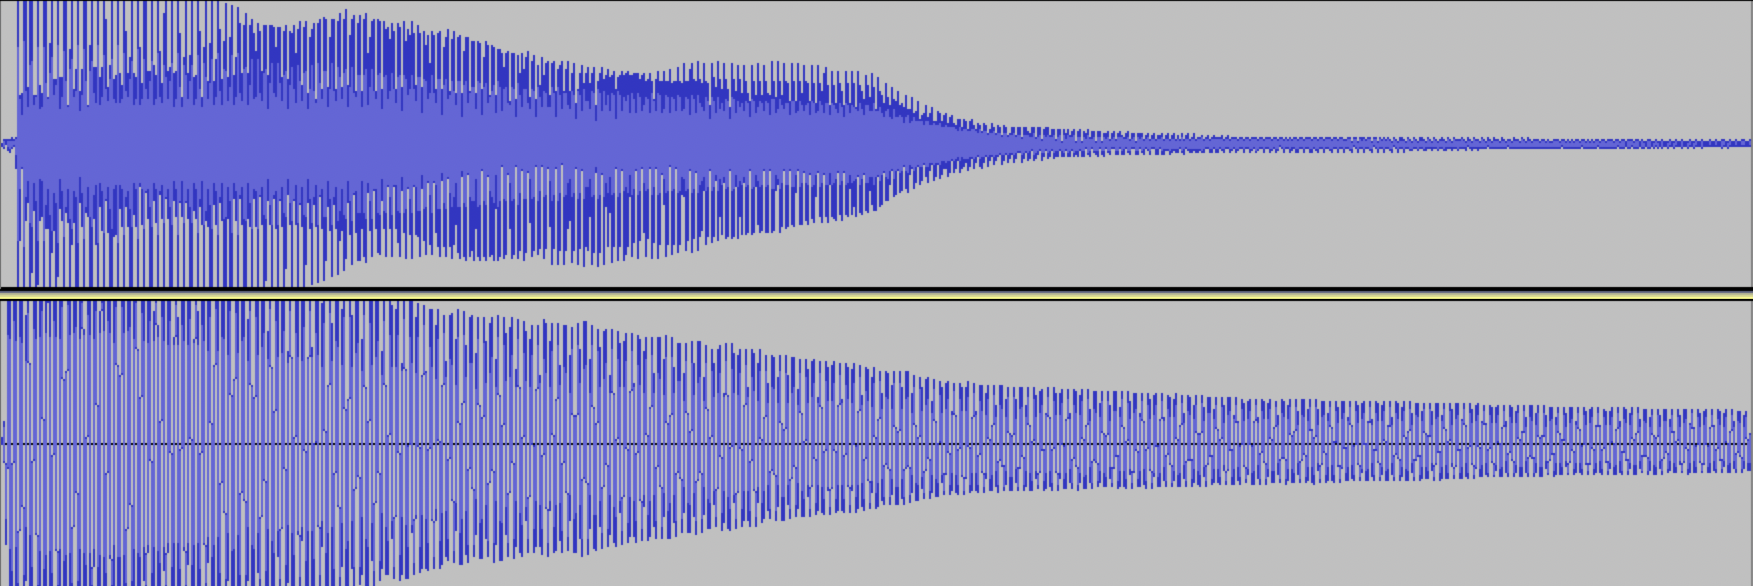
\includegraphics[width=0.7\hsize]{figure/c4_guitar_harp.png}
\caption{ギターとハープの音色}
\label{fig:guitar_harp_comp}
\end{center}
\end{figure}

音の高さと大きさが同じであっても異なった音として人間には知覚される。この違いを音色と呼ぶ。

図\ref{fig:guitar_harp_comp}では、上側はギターの音波,下側はハープの音波で同じ高さかつ同じ大きさである。この音波の波形の違いが音色の違いを作り出す。
